%
% This is the LaTeX template file for lecture notes for EE 382C/EE 361C.
%
% To familiarize yourself with this template, the body contains
% some examples of its use.  Look them over.  Then you can
% run LaTeX on this file.  After you have LaTeXed this file then
% you can look over the result either by printing it out with
% dvips or using xdvi.
%
% This template is based on the template for Prof. Sinclair's CS 270.

\documentclass[twoside]{article}
\usepackage{graphics}
\usepackage{listings}
\usepackage{graphicx}
\setlength{\oddsidemargin}{0.25 in}
\setlength{\evensidemargin}{-0.25 in}
\setlength{\topmargin}{-0.6 in}
\setlength{\textwidth}{6.5 in}
\setlength{\textheight}{8.5 in}
\setlength{\headsep}{0.75 in}
\setlength{\parindent}{0 in}
\setlength{\parskip}{0.1 in}

%
% The following commands set up the lecnum (lecture number)
% counter and make various numbering schemes work relative
% to the lecture number.
%
\newcounter{lecnum}
\renewcommand{\thepage}{\thelecnum-\arabic{page}}
\renewcommand{\thesection}{\thelecnum.\arabic{section}}
\renewcommand{\theequation}{\thelecnum.\arabic{equation}}
\renewcommand{\thefigure}{\thelecnum.\arabic{figure}}
\renewcommand{\thetable}{\thelecnum.\arabic{table}}

%
% The following macro is used to generate the header.
%
\newcommand{\lecture}[4]{
   \pagestyle{myheadings}
   \thispagestyle{plain}
   \newpage
   \setcounter{lecnum}{#1}
   \setcounter{page}{1}
   \noindent
   \begin{center}
   \framebox{
      \vbox{\vspace{2mm}
    \hbox to 6.28in { {\bf EE 382C/361C: Multicore Computing
                        \hfill Fall 2016} }
       \vspace{4mm}
       \hbox to 6.28in { {\Large \hfill Lecture #1: #2  \hfill} }
       \vspace{2mm}
       \hbox to 6.28in { {\it Lecturer: #3 \hfill Scribe: #4} }
      \vspace{2mm}}
   }
   \end{center}
   \markboth{Lecture #1: #2}{Lecture #1: #2}
   %{\bf Disclaimer}: {\it These notes have not been subjected to the
   %usual scrutiny reserved for formal publications.  They may be distributed
   %outside this class only with the permission of the Instructor.}
   \vspace*{4mm}
}

%
% Convention for citations is authors' initials followed by the year.
% For example, to cite a paper by Leighton and Maggs you would type
% \cite{LM89}, and to cite a paper by Strassen you would type \cite{S69}.
% (To avoid bibliography problems, for now we redefine the \cite command.)
% Also commands that create a suitable format for the reference list.
\renewcommand{\cite}[1]{[#1]}
\def\beginrefs{\begin{list}%
        {[\arabic{equation}]}{\usecounter{equation}
         \setlength{\leftmargin}{2.0truecm}\setlength{\labelsep}{0.4truecm}%
         \setlength{\labelwidth}{1.6truecm}}}
\def\endrefs{\end{list}}
\def\bibentry#1{\item[\hbox{[#1]}]}

%Use this command for a figure; it puts a figure in wherever you want it.
%usage: \fig{NUMBER}{SPACE-IN-INCHES}{CAPTION}
\newcommand{\fig}[3]{
			\vspace{#2}
			\begin{center}
			Figure \thelecnum.#1:~#3
			\end{center}
	}
% Use these for theorems, lemmas, proofs, etc.
\newtheorem{theorem}{Theorem}[lecnum]
\newtheorem{lemma}[theorem]{Lemma}
\newtheorem{proposition}[theorem]{Proposition}
\newtheorem{claim}[theorem]{Claim}
\newtheorem{corollary}[theorem]{Corollary}
\newtheorem{definition}[theorem]{Definition}
\newenvironment{proof}{{\bf Proof:}}{\hfill\rule{2mm}{2mm}}

% **** IF YOU WANT TO DEFINE ADDITIONAL MACROS FOR YOURSELF, PUT THEM HERE:

\begin{document}
%FILL IN THE RIGHT INFO.
%\lecture{**LECTURE-NUMBER**}{**DATE**}{**LECTURER**}{**SCRIBE**}
\lecture{21}{November 8}{Vijay Garg}{Edward Clinton, TEC553}
%\footnotetext{These notes are partially based on those of Nigel Mansell.}

\section{Agenda}
This lecture deals with transaction memory.
We will focus on 4 characteristics of transactions:
\begin{itemize}
\item{A - Atomicity}
\item{C - Consistency}
\item{I - Isolation}
\item{D - Durability}
\end{itemize}

Transaction memory: we will look at Atomicity, Consistency and Isolation, not worried about Durability

% **** YOUR NOTES GO HERE:

% Some general latex examples and examples making use of the
% macros follow.  
%**** IN GENERAL, BE BRIEF. LONG SCRIBE NOTES, NO MATTER HOW WELL WRITTEN,
%**** ARE NEVER READ BY ANYBODY.
\section{Introduction}
A transaction is a sequence of events that appears indivisible and instantaneous to an outside observer and has four properties:
\begin{itemize}
\item Atomicity: All constituent actions in a transaction complete successfully, or none of these actions appear to start executing.
\item Consistency: A transaction can modify the state of the world, i.e. data in a database or memory. These changes should leave this state consistent. If the transaction completes successfully, then the system will be in a valid state. If an error occurs then any change will be rolled back. For example, when transfering money from account A to account B, the system is consistent if the total of all accounts is constant. If an error occurs after removing money from account A but before adding it to account B, the system is no longer consistent since the total would have changed (money disappeared). By rolling back the removal from account A, the system will be back in a consistent state.


\item Isolation: Each transaction produces a correct result, regardless of which other transaction are executing concurrently. (i.e. the system state would be obtained if transactions were executed serially)
\item Durability: Once a transaction commits, its result is permanent (stored in a durable media such as disk) 
\end{itemize}

Transactions is a language construct that discharges programmers from the management of synchronization issues. (synchronization constructs such as locks are hidden from the programmer). 

\section{Serializability}
The correctness condition in transactions is called serializability. Serializability states that the concurrent execution of transactions is equivalent to some serial execution of all transactions. In other words, it appears that one transaction finishes before the next transaction starts.
For example, if $T_1$, $T_2$ and $T_3$ execute concurrently, the net result should be equivalent as if these transactions ran sequentialy such as: $T_2 -> T_1 -> T_3$ or $T_3 -> T_2 -> T_1$ etc.. (there are n! possibilities).

\section{Transaction construct}
In the database world, the programmer does not have to worry about using locks for synchronization. Synchronization is all taken care of by the underlying system.
To enable transactions we add one additional construct to import in a programming language as follows:

\begin{lstlisting}
atomic{
//do whatever you want
	x:=2;
    while(){
    	//do stuff
    };
}
\end{lstlisting}

This atomic construct assures that the block is executed as one single step such that a process running concurrently can only observe a state that is either before or after the atomic block executes.

At first this construct may seem equivalent to the java synchronized block. The difference is that the synchronized block locks the object implementing the synchronized method such that operations in the synchronized blocks cannot be interleaved. However in transactions, its OK to interleave operations inside an atomic block as long as the effect is the same as if each block executed separately. 

Another difference is that transactions use speculative (optimistic) execution to execute multiple transactions in parallel (hoping that nothing bad happens). If contention is low then there is a good chance that nothing bad will happen. If there is a conflict between two atomic blocks the system will resolve it using aborts and roll-backs.

Some issues of locks vs transactions:
\begin{itemize}
\item \textbf{Deadlocks} , There is no notion of deadlocks in TM. If there is a conflict between some transactions (atomic blocks). The system will resolve it using aborts. Aborts are not available in Java synchronization.
\item \textbf{Composability problem}. Given two data structures Q1 and Q2 we perform following operation atomically:
\begin{lstlisting}
atomic{
x = q1.deq();
q2.enq(x);
}
\end{lstlisting}

Invariant: No process shall find a state where x is not in q1 nor q2 (i.e. X has to be in q1 or q2 and not in both). In TM, this is achieved trivially by using atomic block. If using locks, this problem is non-trivial. Locks cannot be easily composed. In Queue implementations based on monitors, each method acquires the lock internally, so it is essentially impossible to combine two method calls this way.

\end{itemize}

\section{Opacity}
Opacity is a correctness condition for TMs. An execution satisfies opacity if all the committed transactions and the read prefix of the aborted transactions appear as if they have been executed serially in agreement with real-time occurrence order. Opacity can be viewed as an extension of serializability with the additional requirement that even non-committed transactions are prevented from accessing inconsistent states.

For example:
\begin{lstlisting}
x = 1;
y = 0;

atomic{
x++;
y++;
}

atomic{
z = z/(x - y) //<- can raise a divide by zero exception
//zombie transaction, read values that are impossible (ex x == y)
//if all transactions occured serially

}

\end{lstlisting}

Opacity guarantees that x != y since x != y is true in all the consistent global states of the multiprocess program (no transaction can read values from an inconsistent global state). 

\section{Implementation and Algorithm}
There are multiple implementations (ex Deuce STM , Hardware Transaction memory (HDM) for small transactions ). Current state of the art : no algorithms are currently used because of their high overhead (higher than locking , or lock free). But there is optimism that transactions will become useful someday.

In HDM, the idea is that since in a normal machine all updates are stored in the cache and not in main memory (cache block is written-back to main memory before getting evicted, only true for write-back cache) the abortion of a transaction can be implemented by not writing the cache block(s) back to main memory.

We will focus on an STM (software transaction memory) system called  TL2 (transactional locking 2) due to D. Dice, O. Shalev, and N. Shavit (2006). This STM system statisfies the opacity consistency condition.
The TL2 algorithm is posted on canvas.

The TL2 algorithms uses locks (lock usage is minimized). Locks are used when a transaction is about to be committed to check if the states are consistent and to determine if the transaction needs to be committed or aborted. TL2 also uses atomic instructions.

\textbf{Properties and control variables of TL2:}
\begin{itemize}
\item CLOCK: clock is a fetch and add register initialized to 0 and is used as a logical clock to measure the progress of the system. It represents the number of transactions that have been committed so far.
\item All registers are MWMR atomic registers. Each register has two fields: \textit{value}, which contains the value of the register, \textit{date} which contains the date of its last update. A lock is associated with each register. 
\item Each process has two local variables \textit{lrs(T)} and \textit{lws(T)} where T is the transaction currently executing. \textit{lrs(T)} (local read set) contains the names of all registers read by T until now. \textit{lws(T)} (local write set) contains all the registers written up to now.

\end{itemize}

We will look at an implementation of a \textit{begin} , \textit{end} transaction and how to read and write objects.

\begin{lstlisting}
begin()
{
lst(T) <- {} ; rst(T) <- {} ;
birthdate(T) <- CLOCK + 1 ; 
return;
}
\end{lstlisting}

When reading an object we first read it into a local copy

\begin{lstlisting}
X.readT()
{
if(there is a local copy lc(XX) of XX){
	then return(lc(XX).value)
    }
    else lc(XX) <- copy of XX read from the shared memory;
    if(lc(XX).date < bitrhdate(T)){
    	then lrst <- lrst U {X}; return(lc(XX).value)
        }
        else return(abort)
}

\end{lstlisting}
If the date of the register is not less than the birth date of the transaction then we must abort the transaction to guarantee opacity. A transaction cannot read from the future.

\begin{lstlisting}
X.write(V)
{
if(there is no local copy of XX) then allocate local space lc(XX) for a copy
lc(XX).value <- v ; lwstt <- lwst U {X};
return(ok) //write never aborts
}

\end{lstlisting}

If a transaction reaches its last statement without having been previously aborted, it invokes the \textbf{commit} operation. That operation decides the fate of T by returning commit or abort.

\begin{lstlisting}
try_to_commit()
{
lock all the objects in (lrst U lwst);
for each X in lrst do
{
	//the date of XX is read from the shared memory
    if XX.date >= birthdate(T) then release all the locks; return abort
}
write_date <- CLOCK.fetch&add();
for each X in lwst do XX <- (lc(XX).value, write_date) 
release all the locks; return commit


}

\end{lstlisting}

If the read validation succeeds (as explained above), the process has to compute the new date that has to be associated with all the writes issued by T. All written local copies are then stored to shared memory.

This algorithm is slow due to all the copy overhead and local copy write back. When using locks, there is isn't a copy overhead.

\section{Intro to Java Streams}
Stream is a JAVA abstraction introduced to JAVA SE 8. 
A stream is a sequence of aggregate operations as presented below.
\begin{figure}[h]
\caption{}
\centering
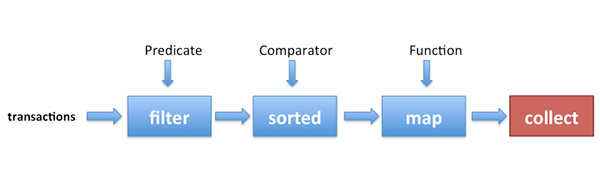
\includegraphics[width=0.9\textwidth]{2179048.png}
\begin{lstlisting}
List<Integer> transactionsIds = 
    transactions.stream()
                .filter(t -> t.getType() == Transaction.GROCERY)
                .sorted(comparing(Transaction::getValue).reversed())
                .map(Transaction::getId)
                .collect(toList());
\end{lstlisting}
\end{figure}

Figure 21.1 illustrates the Java SE 8 code. First, we obtain a stream from the list of transactions (the data) using the stream() method available on List. Next, several operations (filter, sorted, map, collect) are chained together to form a pipeline, which can be seen as forming a query on the data. Stream operations return streams themselves

To parallelize the code, we can use parallelStream() instead of Stream()



\section*{References}
\beginrefs
%\bibentry{AGM97}{\sc N.~Alon}, {\sc Z.~Galil} and {\sc O.~Margalit},
%On the Exponent of the All Pairs Shortest Path Problem,
%{\it Journal of Computer and System Sciences\/}~{\bf 54} (1997),
%pp.~255--262.

\bibentry{R12}{\sc M. Raynal}, Concurrent Programming: Algorithms, Principles and foundations (2012), 
pp.~277-289.
\endrefs


\end{document}